% !TEX root = Projektdokumentation.tex

\newglossaryentry{XML External Entitiy} {name={XML External Entitiy-Attacke},description={Eine Attacke, welche gegen einen XML-Input-Parser geht. Sie tritt auf, wenn der XML-Input einen Verweis auf eine externe Server-Ressource enthält, auf welche der Angreifer gar keinen Zugriff haben dürfte, und der Parser dies nicht prüft. \cite{xxe}}}
\newglossaryentry{Refactoring}{name={Refactoring},
	description={Refactoring bezeichnet die manuelle oder automatisierte Strukturverbesserung von Quelltexten unter Beibehaltung des beobachtbaren Programmverhaltens. Dabei sollen die Lesbarkeit, Verständlichkeit, Wartbarkeit und Erweiterbarkeit verbessert werden, mit dem Ziel, den jeweiligen Aufwand für Fehleranalyse und funktionale Erweiterungen deutlich zu senken. \cite{_refactoring_2016}}
}

\todo{Verweis auf Anhang 'Änderungen am Server'}


	





\section{Verbesserung der bestehenden Lösung}

\subsection{\gls{Refactoring} und Fehlerbehebung}

Aufgrund der im Punkt \ref{subsec:eigeneUntersuchungen} vorgenommenen eigenen Untersuchungen des Mobile Quiz entstand eine Liste von zu behebenden Problemen. Diese detaillierte Liste ist im Dokument 'Ergebnisse eigene Tests.pdf' ersichtlich. In diesem Kapitel werden die wichtigsten vorgenommenen Änderungen angeschaut.

\begin{itemize}
	\item Es wurden unterschiedliche Fehlermeldungen bei falscher E-Mail Adresse oder falschem Passwort ausgegeben. Dies wurde aus Sicherheitsgründen geändert. Es wird neu bei einer falschen Eingabe von Passwort oder E-Mail folgende generelle Meldung angezeigt:	
	\begin{figure}[H]
		\centering
		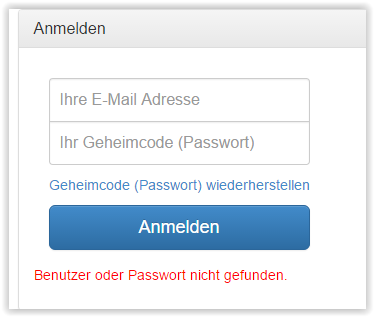
\includegraphics[width=0.5\textwidth]
		{Images/nachher_Email-und-Passwort.PNG}
		\caption{Neu Umgesetzte Fehlermeldung}
	\end{figure}

	\item Wenn an einem Quiz Teilgenommen wird und versucht wird, das Quiz durch klicken auf den Abbrechen-Button zu verlassen, führte das teilweise zu keine Aktion. An was dies lag, ist in folgendem Bild gut ersichtlich. Es wurde nur innerhalb der blauen Markierung auf die Klicks von Benutzer reagiert. Dieser Ausschnitt wurde als Korrekturmassnahme direkt über den Abbrechen-Button platziert.
	\begin{figure}[H]
		\centering
		
\includegraphics[width=0.75\textwidth]
		{Images/CancelButtonProblem.PNG}
		\caption{Screenshot des Problems des Abbrechen-Buttons}
	\end{figure}
	
	\begin{figure}[H]
		\centering
		
\includegraphics[width=0.75\textwidth]
		{Images/CancelButtonFix.PNG}
		\caption{Screenshot der Lösung für das Problem des Abbrechen-Buttons}
	\end{figure}
	
	\item Es wurden diverse Verbesserungen im HTML vorgenommen. Zum Beispiel waren im Registrierungsformular sämtliche Input-Typen auf 'text' gesetzt. Diese wurden entsprechend dem tatsächlich passenden bzw. erwarteten Datentyp angepasst.
	
	Zudem wurde der Doctype-Tag von HTML4 auf HTML5 aktualisiert. Dieser Doctype-Tag teilt dem Browser mit, in welcher Version das HTML geschrieben ist und wie er das Dokument zu interpretieren hat.
	
	\item An den wichtigsten Stellen wurde die gefundene \gls{Cross-Site-Scripting} Schwachstelle behoben. Es gibt allerdings noch Stellen im Mobile Quiz wo diese Schwachstelle nicht behoben wurde. Grundsätzlich müsste jedes Element welches von einem Benutzer (sei es Teilnehmer, Ersteller, Assistent oder Administrator) eingegeben wurde bei seiner Ausgabe so codiert werden, dass es nicht mehr ausgeführt werden kann. Wenn dies nicht gemacht ist, kann ein böswilliger Benutzer von ihm erstellten Code ausführen lassen. Dies kann im schlimmsten Fall zum Verlust von Benutzerdaten und Sessions führen. Damit kann ein Angreifer dann im Namen von anderen Benutzer im System agieren.
	
	\item Bei der Durchführung eines Quizzes wird oben links im Stil X/Y jeweils angezeigt, bei welcher Frage X der totalen Anzahl zu beantwortenden Fragen Y man sich befindet. Allerdings hatte es einen Fehler in der Logik, es wurde bei Zurück-Navigieren ebenfalls nach oben gezählt, womit die Aussage nicht mehr stimmte.
	Die Logik wurde so angepasst, dass dieser Zähler nun in jedem Fall stimmt. 
	
\end{itemize}


\subsection{Frage-Template}

\label{subsec:FrageTemplate}
Die Möglichkeit, Fragen offline zu erstellen und anschliessend hochzuladen, bestand bereits. Unterstützt wurde die Erfassung von Singechoice und Multiplechoice-Fragen. Dazu konnten Fragen in eine CSV-Datei geschrieben werden. Alle korrekten Antworten wurden mit einem Asterisk (Stern-Zeichen) versehen. Eine Multiplechoice-Frage lag vor, wenn mehr als eine Antwort mit einem Asterisk versehen war.

In dieser Arbeit wurde das CSV-Template durch ein Excel-Template abgelöst. Die Gründe dazu sind die folgenden:
\begin{itemize}
	\item Die Regeln für das Erstellen waren einem kleinen Personenkreis bekannt. Sie wurden auf der Webseite nicht beschrieben. Damit die Funktion aber Verbreitung findet, muss die Vorgehensweise öffentlich zugänglich sein.
	
	Es wurde entschieden, ein Excel-Template zum Download auf der Webseite anzubieten. Darin sind alle relevanten Informationen für die Erstellung vorhanden.
	
	\item Werden die Fragen in Excel erstellt und anschliessend daraus eine CSV-Datei generiert, so hat man die Wahl zwischen 3 verschiedenen CSV-Varianten.
	
	Der Excel-Import hingegen unterstützt alle Excel-Dateien mit der Endung .xlsx. Dieses Format ist ab Excel 2007 das Standardformat und daher weit verbreitet.
	\cite{microsoft2016}
	
	\item Das CSV-Template war auf Singlechoice und Multiplechoice - Fragen beschränkt.
	
	Da neue Fragetypen unterstützt werden sollten, wurde eine neue Struktur mittels Excel erarbeitet. Um den Ersteller zu Unterstützen wurde mit Farben und weiteren Funktionen gearbeitet, welche durch CSV nicht unterstützt werden.
\end{itemize}

Ein Beispiel des ursprünglichen Formats sowie des neuen Excel-Templates ist im Anhang, im Kapitel 19 Details zur Lösungsfindung, ersichtlich.

Der neue Template-Import wurde mit PHPExcel \cite{phpexcel} umgesetzt. Diese PHP-Library war bereits im Projekt eingebunden und wird dazu verwendet, die Rangliste aller Teilnehmenden eines Quiz zu Exportieren. Die neue Logik befindet sich hauptsächlich in der neu erstellen Datei 'importExcel.php'.

Bei PHPExcel gab es bis zur Version 1.7.9 eine \gls{XML External Entitiy} - \gls{Vulnerability}. Dadurch war es Remote-Angreifern möglich, beliebige Dateien auf dem Server zu lesen oder eine Denial-of-Service - Attacke durchzuführen. \cite{cvedetails_phpexcel} %TODO Remote und Denial-of-Service erklären
Da bei MobileQuiz allerdings die Version 1.8.0 verwendet wird, ist dies nicht mehr möglich. Es wurde mit dem Wissen von InfSi3 versucht eine solche Attacke durchzuführen, was ebenfalls zum Ergebnis führte, dass diese Sicherheitslücke nicht mehr vorhanden ist. %TODO InfSi3 erklären

\todo{Bildupload mit Excel beschreiben
	https://github.com/dwin94/mobilequiz\_v3/commit/3fe09578311f3e20b5933b71dad546830c321ed0}

\section{Neuerungen}

\subsection{Fragen mit Bildern}

\subsubsection{Hochladen und Entfernen eines Bildes}
Bei jedem Fragetyp ist es neu möglich ein Bild zu hinterlegen. Die Funktion des Bild-Uploads auf den Server bestand bereits, wurde aber erweitert.
\\
\\
Beim Hochladen des Bildes wurde zuvor eine Fehlermeldung ausgegeben, wenn ein Bild eine Grösse von über 20 Megabyte überstieg. Diese Limite wurde herabgesetzt, weil ein Bild von dieser Grösse lange benötigt, bis es heruntergeladen werden kann. Unten ist ein Vergleich von Downloadzeiten aufgeführt, bei verschiedenen Dateigrössen. Die Downloadgeschwindigkeit ist die durchschnittliche Downloadgeschwindigkeit der Swisscom-Kunden, welche anhand von Speedtests der cnlab AG \cite{cnlab_speedtest} ermittelt wurde. Es wurden die Swisscom-Kunden gewählt, weil die Anzahl der User dort am grössten war. \\


\begin{tabular}{|c|c|c|}
	\hline 
	Dateigrösse & Downloadgeschwindigkeit & Benötigte Zeit \\ 
	\hline 
	20 MB & 33,1 Mbit/s & 4,8 s \\ 
	\hline 
	5 MB & 33,1 Mbit/s & 1,2 s \\ 
	\hline 
	800 KB & 33,1 Mbit/s & 0,2 s \\ 
	\hline 
\end{tabular}\\

Falls ein Bild nun 800 Kilobyte übersteigt, so wird es so lange komprimiert, bis seine Dateigrösse darunterliegt. Dies wird durch die PHP-Funktion 'imagecopyresampled' erreicht. Als Code-Vorlage diente das Beispiel von www.williseiler.ch \cite{willis_php}. \\

Weiter gibt es Grössenbeschränkungen von Apache selbst \cite{stackoverflow_largeFilePHP}. Im File 'php.ini' können folgende drei Werte definiert werden:
\begin{itemize}
	\item upload\_max\_filesize: Legt die maximale Dateigrösse für eine Upload-Datei fest. Der Standardwert liegt bei 2 MB.
	\item post\_max\_size: Legt die maximale Grösse aller POST-Daten zusammen fest. Der Standardwert liegt bei 8 MB.
	\item max\_file\_uploads: Legt die maximale Anzahl aller Dateien fest, welche auf einmal hochgeladen werden können. Der Standardwert liegt bei 20 Dateien.
\end{itemize}

Werden via Excel-Template 10 Fragen mit je einem Bild à 1 Megabyte hochgeladen, so ist dies mit der Standardkonfiguration nicht möglich. Diese wurde deshalb folgendermassen angepasst:
\begin{itemize}
	\item upload\_max\_filesize: Neu 5 MB. Grössere Dateien benötigen zu lange für den Upload, allerdings soll der Benutzer nicht nur auf kleine Grössen beschränkt sein. Deshalb wurde von der 2MB-Standardgrösse abgewichen.
	\item post\_max\_size: Neu 25 MB. Bei dieser Grösse beträgt die Uploadzeit bei einer Geschwindigkeit von 15 Mbit/s 13 Sekunden. Dies ist die Durchschnittliche Uploadgeschwindigkeit von Swisscom-Kunden, welche beim Speedtest der cnlab AG \cite{cnlab_speedtest} erreicht wurde. Diese Messungen umfassen jedoch auch Mobile-Messungen mit Smartphones. Da die Uploads der Frage-Templates aber eher von Computern und Laptops erfolgen, welche dank LAN und WLAN eine höhere Uploadgeschwindigkeit aufweisen, ist diese Uploadzeit eher geringer. Der Benutzer sollte sich zudem bewusst sein, dass der Upload bei so vielen Dateien einige Zeit in Anspruch nimmt.
	Auf der anderen Seite soll der Benutzer aber auch nicht eingeschränkt werden. Es soll möglich sein, gleichzeitig 20 Fragen mit Bildern à 1 MB sowie 1 Frage mit einem grösseren Bild plus Excel-Template hochzuladen.
	\item max\_file\_uploads: Neu 25 Dateien. Der Standard-Wert wird nur leicht angehoben, da es möglich sein soll 20 Fragen mit Bildern gleichzeitig zu erstellen. Damit würde das Maximum von 20 Dateien nicht ausreichen.
\end{itemize}

Beim Upload wird das mit folgendem Dateinahmen im Ordner 'uploadedImages' abgelegt: 'question\_Datum(Tag\_Monat\_Jahr\_Stunde\_Minute\_Sekunde\_\_SessionId.Dateityp'.
\\
\\
Das Excel-Template für die Frage-Erstellung wurde ebenfalls erweitert, dass auch Fragen mit Bildern erstellt werden können. Dazu wurde eine neue Spalte eingefügt, bei welcher man den Bildnamen inklusive Endung einträgt. Die Bilder müssen sich dabei im gleichen Ordner wie das Template befinden. Anschliessend wird der gesamte Ordner hochgeladen.

Es war dabei nicht möglich, nur die Excel-Datei alleine hochzuladen und anschliessend die Bilder selbstständig zu holen. Dies wäre bezüglich der Sicherheit höchst bedenklich.
\\
\\
Wird eine Frage gelöscht, so wird nebst dem Datenbankeintrag neu auch das Bild vom Server entfernt.


\subsubsection{Änderungen am Server}
\textbf{Wichtig:} 
Für den Server-Upload müssen die folgenden zwei Dinge gegeben sein:
\begin{itemize}
	\item Die PHP-Library 'GD' muss für die Bildverarbeitung installiert sein. Ob dies der Falls ist kann mittels PHPInfo() oder nachfolgendem Code festgestellt werden. \cite{zoopable.com} Sollte 'GD' nicht installiert sein, so ist unten ebenfalls der Installationsbefehl aufgeführt. \cite{askubuntu.com_php_extension}
\end{itemize}
\begin{lstlisting}
<?php
if (extension_loaded('gd') && function_exists('gd_info')) {
echo "PHP GD library is installed on your web server";
}
else {
echo "PHP GD library is NOT installed on your web server";
}
?>

sudo apt-get install php5.6-gd
\end{lstlisting}

\begin{itemize}
	\item Die Childprozesse des Apache-Servers, welche die Anfragen beantworten, benötigen Schreibrechte auf den Upload-Ordner. Ob dies gegeben ist, kann mittels folgendem Befehl überprüft und geändert werden. \cite{askubuntu.com_permissions} 
\end{itemize}
\begin{lstlisting}
ps -ef | grep apache | grep -v grep
\end{lstlisting}

\begin{lstlisting}
root      5001     1  0 07:21 ?    00:00:00 /usr/sbin/apache2 -k start
www-data  5021  5001  0 07:21 ?    00:00:00 /usr/sbin/apache2 -k start
www-data  5022  5001  0 07:21 ?    00:00:00 /usr/sbin/apache2 -k start
www-data  5023  5001  0 07:21 ?    00:00:00 /usr/sbin/apache2 -k start
\end{lstlisting}

Ist die Ausgabe wie oben ersichtlich, so werden die Anfragen von Prozessen der Benutzergruppe 'www-data' beantwortet. Die Schreibrechte an diese Gruppe können wie folgt vergeben werden:
\begin{lstlisting}
chgrp www-data /path/to/mydir
chmod g+w /path/to/mydir
\end{lstlisting}




\subsubsection{Anzeige eines Bildes}
Das Bild sollte beim Anzeigen der Frage gross genug dargestellt werden. Auf dem Computer war dies kein Problem, da ein Browserfenster genug Platz dazu bot, bei einem Smartphone hingegen war dieser beschränkt. Deshalb wurde die Anzeige so umgesetzt, dass das Bild beim Klick darauf auf dem ganzen Bildschirm dargestellt wird. Dies wurde mit Photoswipe \cite{photoswipe} umgesetzt, welches von GitHub \cite{github_photoswipe} bezogen wurde. Photoswipe ist eine JavaScript-Library, welche es ermöglicht, Bildgalerien auf Websites darzustellen. Sie unterstützt unter anderem Touch-Gesten und Zoom. So ist es kein Problem, ein Bild mit vielen Details darzustellen.

Nachfolgend ist zu sehen, wie eine Frage mit Bild in verschieden Situationen angezeigt wird.

\begin{figure}[H]
	\centering
	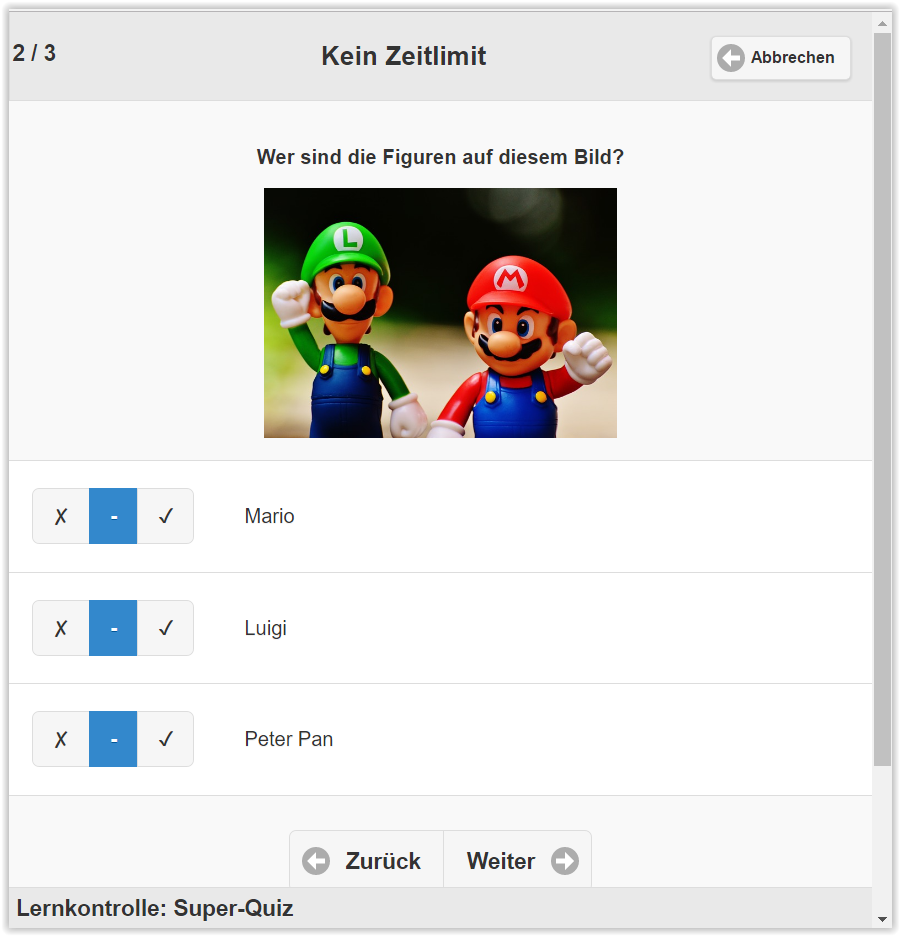
\includegraphics[width=0.75\textwidth]{Images/Frage-Bild_Anzeige_PC.PNG}
	\caption{Anzeige des Frage-Bildes am Computer}
	Quelle: mobilequiz.ch / Fragebild: https://pixabay.com/de/mario-luigi-figuren-lustig-bunt-1558012/
\end{figure}

\begin{figure}[H]
	\centering
	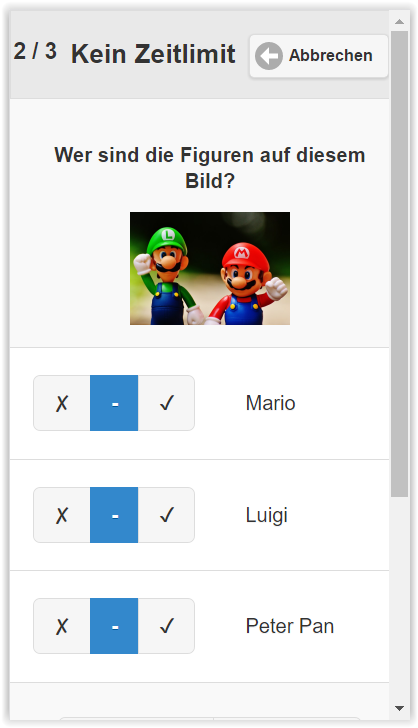
\includegraphics[width=0.3\textwidth]{Images/Frage-Bild_Anzeige_Mobile.PNG}
	\caption{Anzeige des Frage-Bildes auf dem Smartphone}
	Quelle: mobilequiz.ch / Fragebild: https://pixabay.com/de/mario-luigi-figuren-lustig-bunt-1558012/
\end{figure}

\begin{figure}[H]
	\centering
	
\includegraphics[width=0.3\textwidth]{Images/Frage-Bild_Anzeige_Mobile_Full.PNG}
	\caption{Fullscreen-Anzeige des Frage-Bildes auf dem Smartphone}
	Quelle: mobilequiz.ch / Fragebild: https://pixabay.com/de/mario-luigi-figuren-lustig-bunt-1558012/
\end{figure}

Da sich eine Frage, bei welcher ein Bild hochgeladen wird, oft auf Inhalte aus dem Bild bezieht, wurde auch für die Auswertungsseite eine Bild-Anzeige implementiert. Somit können die Auswertungen besser nachvollzogen werden.

Ein Beispiel einer solchen Auswertung ist unten dargestellt.

\begin{figure}[H]
	\centering
	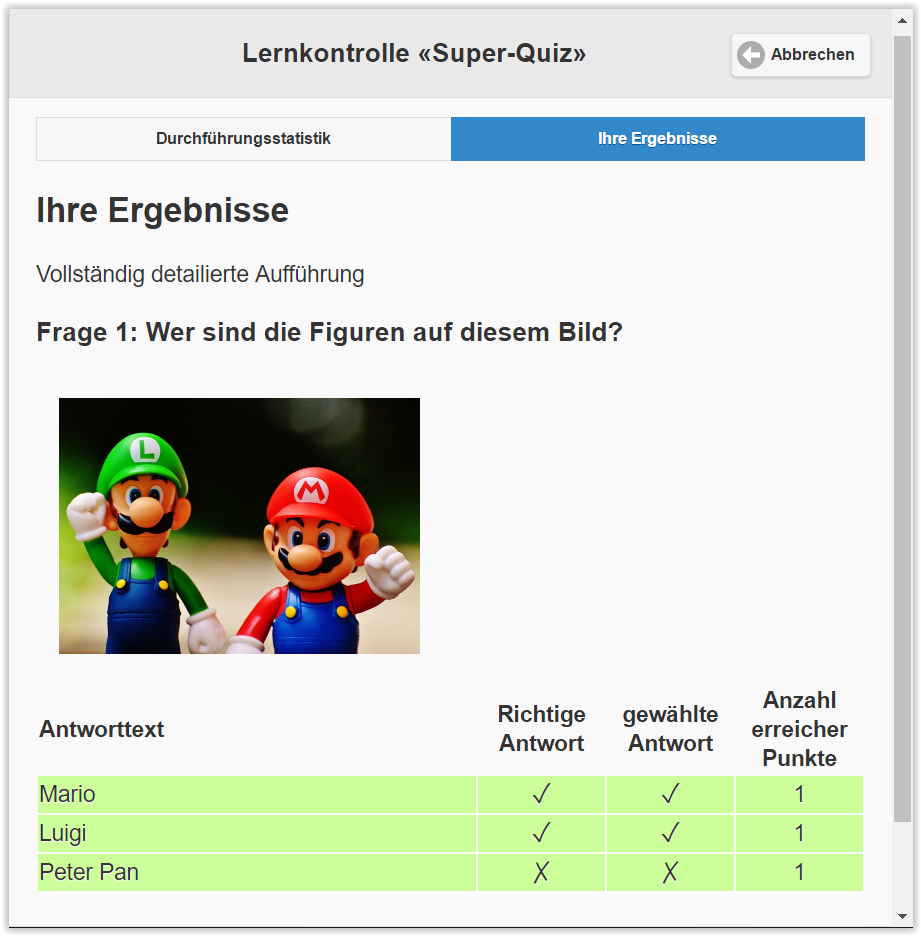
\includegraphics[width=0.75\textwidth]{Images/Quiz-Auswertung_Anzeige.PNG}
	\caption{Auswertungs-Anzeige des Frage-Bildes am Computer}
	Quelle: mobilequiz.ch / Fragebild: https://pixabay.com/de/mario-luigi-figuren-lustig-bunt-1558012/
\end{figure}

Weiter wurde die Generierung des PDF-Aufgabenblattes und Lösungsblattes ergänzt, damit auch dort die Bilder angezeigt werden. Hat man unterwegs kein Internet, so kann man sich die Fragen damit auch vorgängig herunterladen und im Zug anschauen.








\newpage
\subsection{Feedback an Quiz-Ersteller}
Bei der Ausarbeitung von neuen Fragetypen kam die Idee einer Freitext-Frage auf. Bei diesem Fragetyp sind keine Antwortmöglichkeiten vorgegeben, stattdessen schreibt der Teilnehmer seine Antworten in ein leeres Textfeld. Das Problem dabei ist aber die Korrektur, da eine korrekte Antwort auf viele verschiedene Wege niedergeschrieben werden kann. Aus diesem Grund wurde beschlossen, diesen Fragetyp nicht umzusetzen, aber die Idee andernorts zu verwenden.

Ist eine Frage unklar gestellt, gibt es Schreibfehler oder andere Verbesserungsmöglichkeiten, so musste dies ein Teilnehmer bis anhin selbst notieren und den Quiz-Ersteller, in den meisten Fällen der Dozent, im Unterricht fragen. Dies setzt aber voraus, dass der Quiz-Ersteller für den Teilnehmer immer ansprechbar ist. Erstellt ein Dozent aus Rapperswil ein Quiz, an welchem Teilnehmer der ganzen Schweiz mitmachen, so besteht diese Möglichkeit nicht.

Dieses Problem wurde nun angegangen. Unter jeder Frage gibt es neu die Möglichkeit einen Kommentar direkt an den Quiz-Ersteller zu senden.

\begin{figure}[H]
	\centering
	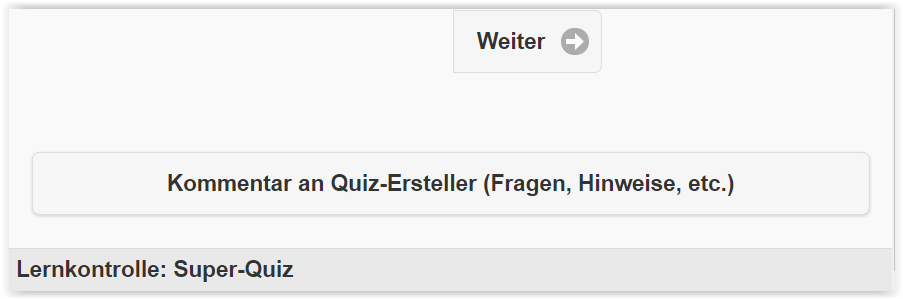
\includegraphics[width=0.75\textwidth]{Images/Feedback-Button.PNG}
	\caption{Feedback-Button}
	Quelle: mobilequiz.ch
\end{figure}

\begin{figure}[H]
	\centering
	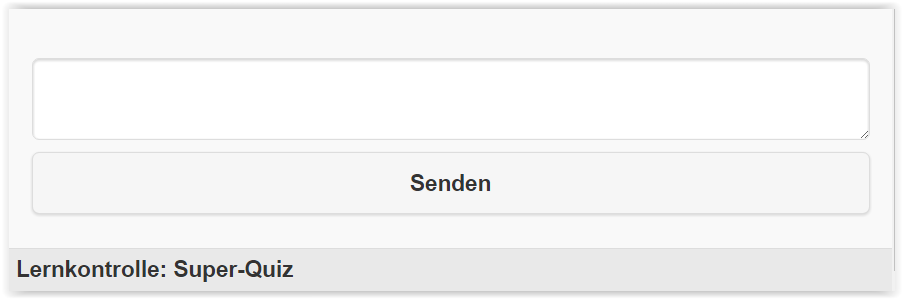
\includegraphics[width=0.75\textwidth]{Images/Feedback-Feld.PNG}
	\caption{Feedback-Feld nach Klick auf Feedback-Button}
	Quelle: mobilequiz.ch
\end{figure}

\begin{figure}[H]
	\centering
	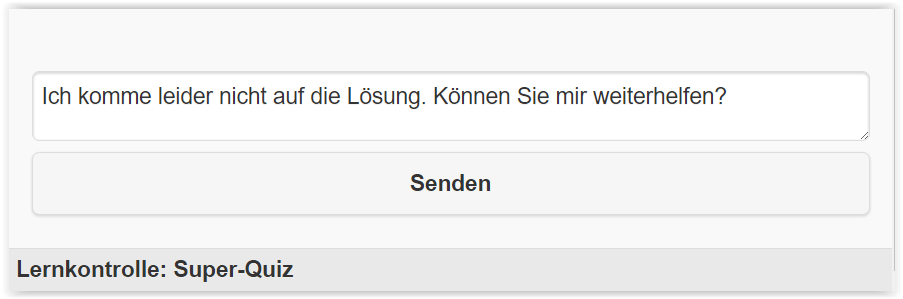
\includegraphics[width=0.75\textwidth]{Images/Feedback-Frage.PNG}
	\caption{Beispielfrage an Quiz-Ersteller}
	Quelle: mobilequiz.ch
\end{figure}

\begin{figure}[H]
	\centering
	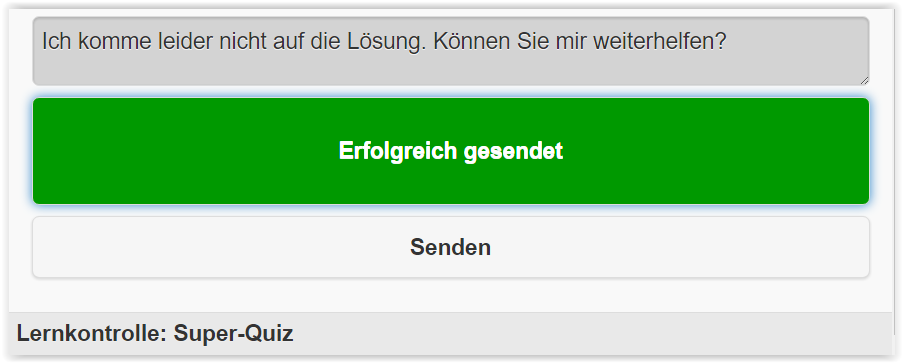
\includegraphics[width=0.75\textwidth]{Images/Feedback-Frage-gesendet.PNG}
	\caption{Feedback versendet nach Klick auf Senden-Button}
	Quelle: mobilequiz.ch
\end{figure}


Nach dem Senden des Feedbacks erhält der Quiz-Ersteller eine E-Mail. Darin ist nicht nur die Frage des Teilnehmers aufgeführt, sondern auch Informationen zum Teilnehmer selbst sowie die gesamte Frage inklusive Antwortmöglichkeiten. Somit hat der Quiz-Ersteller alle Informationen, um auf die Teilnehmer-Frage zu antworten.

\begin{figure}[H]
	\centering
	
\includegraphics[width=0.9\textwidth]{Images/Feedback-Mail_Quiz-Ersteller.PNG}
	\caption{E-Mail an Quiz-Ersteller}
	Quelle: mobilequiz.ch
\end{figure}

Der Teilnehmer selbst erhält ein Bestätigungsmail mit den gleichen Informationen, wie sie auch der Quiz-Ersteller erhält.

\begin{figure}[H]
	\centering
	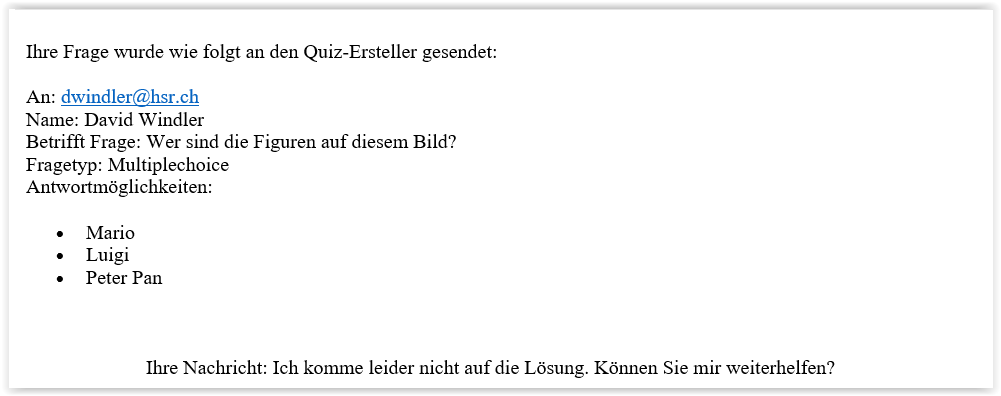
\includegraphics[width=0.9\textwidth]{Images/Feedback-Mail_Teilnehmer.PNG}
	\caption{Bestätigungs-E-Mail an Teilnehmer}
	Quelle: mobilequiz.ch
\end{figure}




\section{Neue Quiz- und Frageerstellung}
%Wieso wurde umgestellt? intuitiver / Usability-Tests

% Mobile-freundlicher mit accordeon





\subsection{Quiz-Erstellung} %ev. eigene Subsection "Durchführung"
\label{subsec:quiz-erstellung}
%•	Das Token bei der Quiz-Teilnahme ist dient als Kurzform zum Link mit der Quiz-Id und ist zudem Datenbank-unabhängig.

%•	Die Implementierung der Durchführung konnte nicht fertiggestellt werden. Die benötigten Informationen für die Fertigstellung werden in der Dokumentation festgehalten.

%asynchron mit ajax -> Meldung 'gespeichert', deshalb wurde auch der Excel-Upload asynchrom gemacht

%asynchrones hinzufügen von neuen fragen aus dem Pool. Ev mit Verweis auf Usability-Testing (Button umbenennen)

\subsection{Frage-Erstellung}
%•	Maximale Anzahl Antwortmöglichkeiten 5? Wenige Fragen haben 6 Möglichkeiten, s. DB-Abfrage
%•	Umsetzung Frage-Screen: Änderungen werden sofort nach Ändern eines Feldes gespeichert, nicht erst beim Tab-Wechsel oder beim Verlassen des Erfassungs-Screens. Somit erübrigt sich auch eine automatische Speicherung alle 30 Sekunden.
%•	Die Fragen, welche mehr als 6 Antwortmöglichkeiten haben, werden per E-Mail an P. Heinzmann geschickt. Er schreibt den Studenten, welche Antwortmöglichkeiten gelöscht werden sollen. Die Studenten passen anschliessend die Datenbank an.
%o	Das hochgeladene Bild soll auch bei den Antwortmöglichkeiten angezeigt werden. Dies hilft bei deren Erfassung, da sich die Antwortmöglichkeiten häufig auf das Bild beziehen.
%o	Wird die Möglichkeit «Single-Choice-Frage» ausgewählt, sollen anstatt Checkboxen Radio-Buttons angezeigt werden (wenn es möglich ist).
%o	Komplett leere Fragen und leere Quizzes sollen nicht gespeichert werden.
%o	Beim Reload soll kein neues, leeres Frage-Formular angezeigt werden, sondern es soll in den Edit-Mode gewechselt werden (dasselbe soll beim Quiz gelten).
%•	Es ist dem Benutzer unter Umständen nicht klar, dass alle seine Änderungen sofort gespeichert werden. Es soll deshalb bei jeder erfolgreichen Speicherung eine kurze Meldung «Gespeichert» bzw. «Saved» eingeblendet werden. Diese könnte im unteren rechten Fensterrand erscheinen. Allenfalls bietet Bootstrap eine solche Lösung bereits an.

%improved Formcheck -> Bild einfügen

%asynchroner Bildupload mit ajax

%- formcheck wird nur noch auf dem client gemacht


%- ev. datenbankskript für update alte statistiken

%Bildbeschreibung bei Bild-Upload anbieten, falls bild nicht geladen oder Screen-Reader


\subsection{Default-Quiz-Einstellungen}
Verweis auf Dokument

%•	Wie in der letzten Sitzung besprochen, soll es bei der Durchführung die Möglichkeit geben, die Einstellungen auf den Standard zurückzusetzen. Es wurde nun beschlossen, dass dazu ein Button «Auf Standard zurücksetzen» angezeigt wird. Hat das Feld bereits den Standard-Wert, so ist der Button ausgegraut und kann nicht geklickt werden. Beinhaltet das Feld nicht den Standard-Wert, so sieht der Benutzer beim darüberfahren mit der Maus, welches der Standard-Wert ist und kann diesen durch Klicken übernehmen.


\section{Interessensgruppen und Filterumstellung}
Loggt sich ein Teilnehmer bei Mobile Quiz ein, so soll er möglichst wenige Klicks von seinem zu lösenden Quiz entfernt sein. Dadurch spart er Zeit da, er sich nicht mit Filteroptionen und Suchfeldern auseinandersetzen muss. Doch wie erkennt Mobile Quiz welche Quizzes für den Teilnehmer interessant sind?

Möglich wäre es nachzuschauen, zu welchem Themengebiet der Teilnehmer schon Quizzes gelöst hat und aufgrund dessen die Filterauswahl bereits auf das Themengebiet mit seinen meisten Teilnahmen zu setzen. Das Problem dieser Methode liegt darin, dass sie für neu registrierte Teilnehmer nicht verwendet werden kann.
Aus diesem Grund wurde eine noch einfachere Methode implementiert. Dabei wird bei der Registrierung eines oder mehrere Interessengebiete angegeben. Diese werden dabei vorgemerkt und beim anschliessenden Aufruf aller Durchführungen wird der Themengebiet-Filter entsprechend der Interessensgebiete des Teilnehmers gesetzt. Meldet beispielsweise ein Student von CN1 bei Mobile Quiz an und setzt das Interessengebiet entsprechend, so werden zuerst immer die Quiz-Durchführungen von CN1 angezeigt. Besucht er zu einem späteren Semester das Modul Informationssicherheit 1, so kann er das Interessensgebiet jederzeit in seinen Profileinstellungen ändern.

\begin{figure}[H]
	\centering
	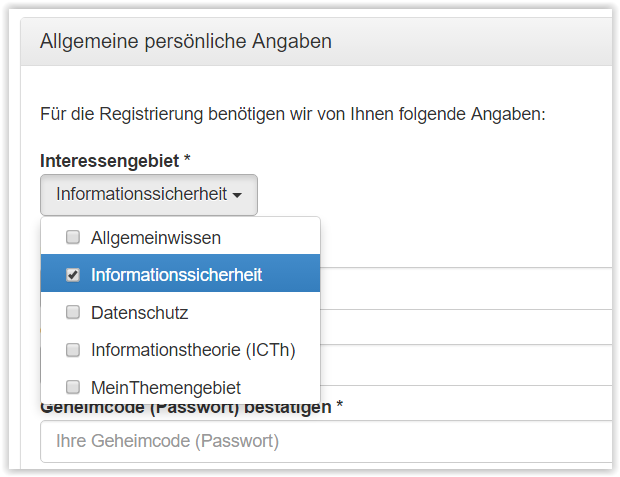
\includegraphics[width=0.5\textwidth]{Images/Themengebiet_Angabe_Registrierung.PNG}
	\caption{Angabe des Interessengebietes bei der Registrierung}
\end{figure}

Wie werden die Interessen der Teilnehmer in der Datenbank abgespeichert? Dazu half die Umstellung der Datenbank, welche es nun zulässt, dass ein Teilnehmer in mehreren Gruppen eingetragen werden kann.
Für jedes Themengebiet wurde eine Interessengruppe erstellt. Gibt ein Teilnehmer ein neues Interesse an, so wird er automatisch zur entsprechenden Interessen-Gruppe hinzugefügt. Interessengruppen werden automatisch mit der Erfassung eines neuen Themengebietes erstellt, beziehungsweise mit dem Entfernen wieder gelöscht und alle Teilnehmer ausgetragen.

\bigskip

Damit ein Teilnehmer mehrere Interessensgebiete angeben kann, war es nötig die Implementierung der Filter zu ändern. Bisher konnte jeweils nur eine Auswahl pro Filter gesetzt werden. Für die Umsetzung wurde die Library 'Bootstrap Multiselect' \cite{bootstrap_multiselect} von David Stutz verwendet. Durch eine Logikumstellung auf dem Server war es anschliessend für Quiz-Durchführungen und Fragen möglich eine Mehrfachauswahl pro Filter zu setzen.

\begin{figure}[H]
	\centering
	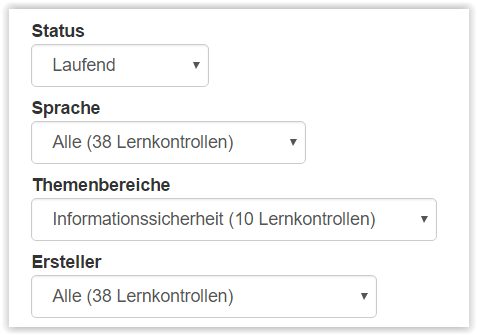
\includegraphics[width=0.5\textwidth]{Images/Alte_Filter_Mobile_Quiz.PNG}
	\caption{Filter der bestehenden Mobile Quiz - Version 3}
	\cite{mobilequiz.ch}
\end{figure}

\begin{figure}[H]
	\centering
	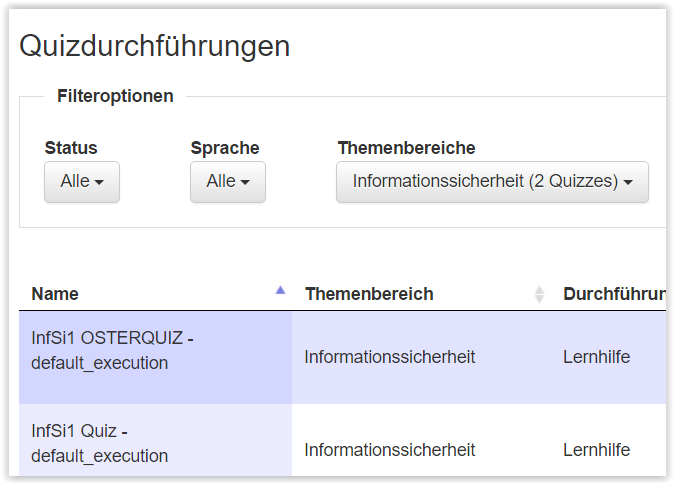
\includegraphics[width=0.5\textwidth]{Images/Neue_Filter_Mobile_Quiz.PNG}
	\caption{Filter der neuen Mobile Quiz - Version}
\end{figure}



\section{Umgestaltung Startseite Teilnehmer / Ersteller}
Filter, Anzeige der Durchführungen statt der einzelnen quizzes

%weniger angezeigte spalten und ersetzung der symbole durch menu mit text glyphicons
%beschreiben, wo dass die glyphicons gespeichert sind -> https://github.com/dwin94/mobilequiz_v3/commit/f4d4417696d31e12925213212342b79d5afeec96


\section{Mobile Ansicht}
%o	Es sollen alle Aktionen in der Mobile-Version dargestellt werden. Dazu müssen einige Aktionen gekürzt oder umgebrochen werden. Bsp: «Lösungsblatt anzeigen / drucken»
% plus andere Seiten, auf denen die Ansicht optimiert wurde -> ev. Teilnahme, Screenshot altes und neues mobile quiz

\section{Schlussprodukt}


